% Foliensatz: "AFu-Kurs nach DJ4UF" von DK0TU, Amateurfunkgruppe der TU Berlin
% Lizenz: CC BY-NC-SA 3.0 de (http://creativecommons.org/licenses/by-nc-sa/3.0/de/)
% Autoren: Lars Weiler <dc4lw@darc.de>

preamble.dk0tu.tex
\usepackage{amssymb}
\subtitle{Organisatorisches 00\\[2em]}
\date{Stand 18.09.2017}
 \begin{document}

\begin{frame}
    \titlepage
    \vfill
    \begin{center}
        \ccbyncsaeu\\
        {\tiny This work is licensed under the \em{Creative Commons Attribution-NonCommercial-ShareAlike 3.0 License}.}\\[0.5ex]
         \tiny Amateurfunkgruppe der Technische Universität Berlin (AfuTUB), DKØTU
         %\includegraphics[scale=0.5]{img/DK0TU_Logo.pdf}
    \end{center}
\end{frame}



\section{Orga}

\subsection{Clubraum CCCB}

\begin{frame}
    \frametitle{Wo finde ich was?}

    \begin{itemize}
      \item $\rightarrow$ Getränkeautomat, bitte Kleingeld mitbringen
      \item $\longrightarrow$ Toiletten
      \item $\looparrowright$ Ausgang und Raucherbereich im Innenhof
    \end{itemize}
\end{frame}


\subsection{DC4LW}

\begin{frame}
  \frametitle{Ausbilder Lars Weiler DC4LW}

  \begin{itemize}
    \item Rufzeichen DC4LW
    \item Ausbildungsrufzeichen DN3CCC
    \item seit 1999 im CCC dabei
    \item seit 2006 Funkamateur
    \item Schwerpunkte: Outdoorfunken, QRP, Portabel, Digimodes, Satellitenfunk
    \item Mitglied auch im DARC e.V.
    \item Referat für Ausbildung, Jugendarbeit, Weiterbildung (AJW) im DARC
    \item fünfter Ausbildungskurs nach Herbst 2013, Sommer 2014, Herbst 2015 und Herbst 2016
  \end{itemize}
\end{frame}

\begin{frame}
  \frametitle{Weitere Ausbilder}

  \begin{itemize}
    \item Andreas DJ3EI
    \item Jörg DC7BWK
    \item Florian DL7MTX
    \item Stefan DD6SW
    \item Loria DL2LJ
    \item Rolf DL1RBC
  \end{itemize}
\end{frame}


\subsection{Kurs}

\begin{frame}
  \frametitle{Zeitraum}

  \begin{center}
    \begin{figure}
      \includegraphics[height=.35\textheight,width=\textwidth,keepaspectratio]{o00/Zeitstrahl_D23_2017.png}
      \caption{Zeitstrahl}
    \end{figure}
  \end{center}

  \begin{itemize}
    \item 18. September bis 18. Dezember 2017: Betriebstechnik, Vorschriften, Technik Klasse E
    \item Optional: Prüfung Klasse E
    \item 08. Januar bis 16. April 2018: Technik Klasse A
    \item Mglw. “Kursfahrt” für ein Wochenende im Frühjahr
    \item Prüfung Klasse A
  \end{itemize}
\end{frame}

\begin{frame}
  \frametitle{Abhängigkeiten}
  \begin{center}
    \begin{figure}
      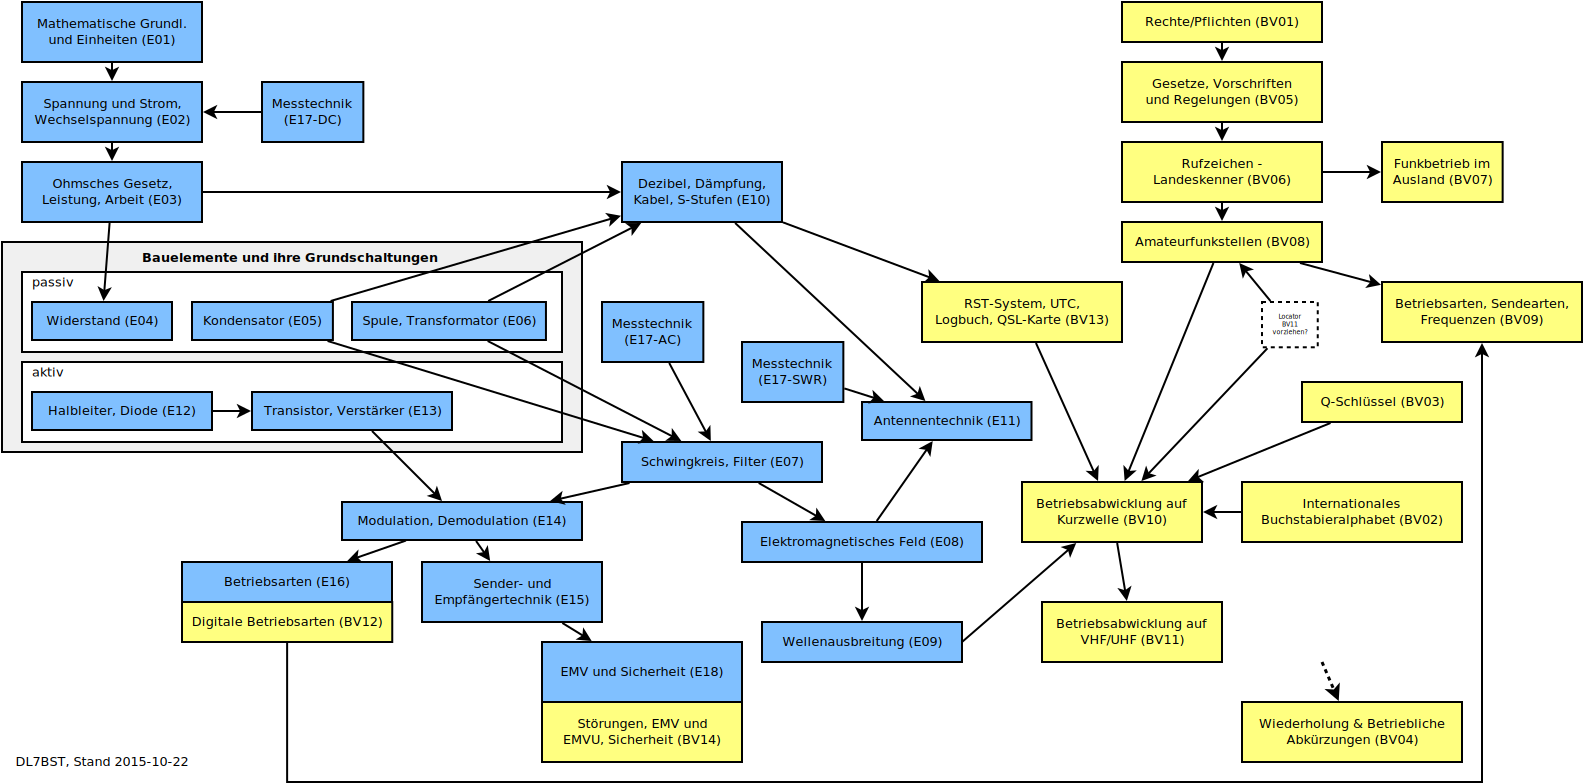
\includegraphics[height=.75\textheight,width=\textwidth,keepaspectratio]{o00/Abhaengigkeitsgraph.png}
      \caption{Abhängigkeitsgraph Klasse E}
    \end{figure}
  \end{center}
\end{frame}


\subsection{Material}

\begin{frame}
  \frametitle{Unterrichtsmaterial}

  \begin{itemize}
    \item nicht-programmierbarer Taschenrechner
    \item Notizblock und Stift für Rechenaufgaben
    \item Funkgerät nicht notwendig
    \item wenn vorhanden, SDR mit Computer und GNU Radio Companion
    \item Sonstiger Bastelkram (frage vorher nach)
    \item ggf. Bücher
      \begin{itemize}
        \item Betriebstechnik und Vorschriften \hyperlink{refs}{\cite{bv}}
        \item Technik Klasse E \hyperlink{refs}{\cite{ale}}
        \item Technik Klasse A \hyperlink{refs}{\cite{ala}}
      \end{itemize}
    \item PDF Lichtblick/Lichtblitz \hyperlink{refs}{\cite{lb}}
    \item Fragenkataloge der BNetzA
  \end{itemize}
\end{frame}


\subsection{Ablauf}

\begin{frame}
  \frametitle{Der Montagabend}

  \begin{itemize}
    \item Tür ab spätestents 17:45 Uhr geöffnet
    \item Beginn um 18:00 Uhr s.t.!
    \item Gegen 19:00 Uhr kurze Pause
    \item Möglicherweise Praxisteil im Anschluss
    \item Offizielles Ende um 20:00 Uhr
    \item Danach offenes Ende im anschließenden Amateurfunkabend
    \item Zeit für Praxisübungen beim Amateurfunkabend
  \end{itemize}
\end{frame}

\subsection{DK0TU}

\begin{frame}
  \frametitle{Zusammenarbeit DK0TU}
  \begin{itemize}
    \item Amateurfunkkurs TU Berlin
    \item Kurs findet ab 26.10. donnerstags ab 16 Uhr statt $\rightarrow$ kann auch besucht werden
    \item \ExternalLink\url{https://www.dk0tu.de/Kurse/AFu-Lizenz/Curriculum/2017_WiSe/}
    \item Gemeinsamer Übungscontest mit Handfunkgeräten
    \item Praktische Ausbildung an Kurzwellenstation
  \end{itemize}
\end{frame}


\subsection{Prüfung}

\begin{frame}
  \frametitle{Die Prüfung bei der BundesNetzAgentur (BNetzA)}

  \begin{itemize}
    \item Es gibt (noch) keine Termine für 2018
    \item Plan: Genügend Anmeldungen einreichen und einen gemeinsamen Termin erhalten
    \item Anmeldebögen in spätestens drei Wochen gesammelt einreichen
    \item Bringe kommende Woche welche mit\ldots
  \end{itemize}
\end{frame}


\subsection{Kosten}

\begin{frame}
  \frametitle{Kursgebühr}

  \begin{itemize}
    \item Der Kurs ist kostenlos
    \item Aber! Bitte \href{https://www.darc.de/der-club/mitgliedschaft/}{\ExternalLink Mitglied im DARC e.V.} werden
      \begin{itemize}
        \item Interessensvertretung
        \item Ortsverband
        \item Ausbildung
        \item Magazin CQ\,DL (auch in digitaler Form)
        \item QSL-Büro
        \item Versicherung
      \end{itemize}
  \end{itemize}
\end{frame}

\begin{frame}
  \frametitle{Kosten}

  \begin{itemize}
    \item einmalig
      \begin{itemize}
        \item Prüfung: 80€ (Klasse E) oder 110€ (Klasse A)
        \item Rufzeichen: 70€
      \end{itemize}
    \item jährlich
      \begin{itemize}
        \item Frequenznutzung, EMV-Abgaben: ca. 25€-35€ (wird alle drei bis vier Jahre eingezogen)
      \end{itemize}
  \end{itemize}
\end{frame}

\subsection{Listen}

\begin{frame}
  \frametitle{Anwesenheits- und Mailingliste}

  \begin{description}
    \item[Anwesenheitsliste] zum Überblick behalten; Nachfragen bei versäumten Unterrichtseinheiten
    \item[Mailingliste] zum Infos rumschicken, Links zu den Präsentationen, Diskussion unter euch
  \end{description}
\end{frame}


%\subsection{Wassersport}

%\begin{frame}
%  \frametitle{Sind Segler oder Motorbootfahrer anwesend?}
%
%  Übungsgruppe für LRC\footnote{Long Range Certificate}, SRC\footnote{Short Range Certificate} und UBI\footnote{UKW-Sprechfunkzeugnis für den Binnenschifffahrtsfunk} im Anchluss an den Kurs
%\end{frame}


\begin{frame}
    \frametitle{Referenzen/Links}
    \hypertarget{refs}{}
    \footnotesize

    \begin{thebibliography}{}
        \bibitem{bv}    Moltrecht, Eckart K.W. DJ4UF, Amateurfunklehrgang Betriebstechnik und Vorschriften, 5.~Auflage 2010, 16,80€, ISBN 978-3881808033 \\
                        \url{http://darcverlag.de/Amateurfunklehrgang-Betriebstechnik-und-Vorschriften}
        \bibitem{ale}   Moltrecht, Eckart K.W. DJ4UF, Amateurfunklehrgang Technik für das Amateurfunkzeugnis Klasse E, 9.~völlig neu bearbeitete Auflage 2014, 18,80€, ISBN 978-3881803649 \\
                        \url{http://darcverlag.de/Amateurfunklehrgang-Technik-fuer-das-Amateurfunkzeugnis-Klasse-E} \\
        \bibitem{ala}   Moltrecht, Eckart K.W. DJ4UF, Amateurfunklehrgang Technik für das Amateurfunkzeugnis Klasse A, 6.~völlig neu bearbeitete Auflage 2012, 19,80€, ISBN 978-3881803892 \\
                        \url{http://darcverlag.de/Amateurfunklehrgang-Technik-fuer-das-Amateurfunkzeugnis-Klasse-A}\\
        \bibitem{lb}	Lindemann, Günter DL9HCG$\dagger$, Lichtblick Klasse A, Lichtblick Klasse E, Lichtblitz \\
          \url{http://www.dl9hcg.a36.de}
    \end{thebibliography}

\end{frame}

% Hier könnte noch eine Kontaktfolie stehen

\end{document}

